\chapter{Materiales}
En este último capítulo vamos a ver como dar color y texturas a los elementos de nuestra escena. Identificaremos cada elemento asignando un entero positivo \(id \in \mathbb{N}\) que será devuelto junto con la distancia a este objeto, es decir, vamos a devolver un \textit{vec2} cuya componente \enquote{x} será la distancia y cuya componente \enquote{y}, el identificador \(id\). Asignaremos la constante \(id=-1\) cuando no hemos trazado ningún objeto.\\\\
En primer luegar, vamos a modificar el \textit{Marcher} para que este pueda devolver ambos valores:

\begin{lstlisting}
// Devolvemos dos elementos, distancia e id.
vec2 SphereMarching(vec3 ojo, vec3 direccion){
    float distancia = 0.0;
    // Realizamos PASOS iteraciones de marching.
    for(int i = 0; i < PASOS; ++i){
        vec3 p = ojo + direccion * distancia;
        // La escena devuelve el radio de la bola y el id del elemento
        vec2 info = escena_sdf(p);
        // info.x contiene la distancia
        if(info.x < EPSILON){
            // info.y contiene el id de un elemento de la escena.
            // Devolvemos la distancia acumulada (o distancia del ojo a la superficie) y el id.
            return vec2(distancia, info.y);
        }
        // incrementamos la distancia
        distancia += info.x;
        if(distancia >= MAXIMO) break;
    }
    // Devolvemos un id desconocido.
    return vec2(MAXIMO, -1);
}
\end{lstlisting}

El vector devuelto con nombre \textit{info} toma los valores directamente de la escena, por lo que vamos a modificar el esquema de nuestra función \enquote{\textit{escena\_sdf}}, este ahora devolverá la distancia más cercana a un objeto y su identificador. El esquema será el siguiente:

\begin{lstlisting}
vec2 escena_sdf(vec3 p){
    // Identificador inicial y la distancia máxima.
    float id = -1.0;
    float min_dist = MAXIMO;
    
    // El esquema es el siguiente para cada figura de nuestra escena.
    // 1. Creamos nuestra primera figura.
    float sdf_0 = ....;
    // 2. Comprobamos que esta figura es la más cercana encontrada hasta el momento.
    if(sdf_0 < min_dist){
        // 2.1 En caso afirmativo, actualizamos los valores.
        // Asignamos el id de esta figura.
        id = 0.;
        // Actualizamos la distancia mínima como la distancia a esa figura.
        min_dist = sdf_0;
    }
    
    // Repetimos este esquema para cada elemento de la escena,
    float sdf_1 = ...;
    if(sdf_1 < min_dist){
        id = 1.;
        min_dist = sdf_1;
    }
    ...
    // Finalmente, devolvemos la distancia mínima y el objeto que la devuelve.
    return vec2(min_dist, id);
}
\end{lstlisting}

Al devolver ahora dos componentes, debemos modificar todas las funciones que llaman a esta función, encontramos el cálculo de la normal:

\begin{lstlisting}
// En escena_sdf, tomamos la primera componente.
vec3 Normal(vec3 rayo){
     // f(x1,...,xn)
     float fxyz = escena_sdf(rayo).x;
     // f(x1,..,xi+h,xn)
     float fxhyz = escena_sdf(rayo + vec3(EPSILON, 0.0, 0.0)).x;
     float fxyhz = escena_sdf(rayo + vec3(0.0, EPSILON, 0.0)).x;
     float fxyzh = escena_sdf(rayo + vec3(0.0, 0.0, EPSILON)).x;
     
     // Utilizamos la definicion de derivadas parciales para devolver el gradiente, que se trata de la normal de la isosuperficie.
     return vec3(
         (fxhyz - fxyz) / EPSILON,
         (fxyhz - fxyz) / EPSILON,
         (fxyzh - fxyz) / EPSILON
     );
}
\end{lstlisting}

Pongamos como ejemplo una sección de un toro y una esfera, el código y apliquemos el esquema utilizado para \enquote{\textit{escena\_sdf}}. El resultado:

\begin{lstlisting}
vec2 escena_sdf(vec3 p){
    // Identificador inicial y distancia máxima.
    float id = -1.0;
    float min_dist = MAXIMO;
    // Toro de radio interno 0.3 y radio externo 0.05.
    // Seccionado por un plano n = -z.
    // Rotamos el toro 
    vec3 pr = rotYZ(p, PI / 4.);
    float sdf_0 = max(
        SDFToro(pr, 0.3, 0.05),
        SDFPlano(p, vec3(0., 0., -1.))
    );
    // Comprobamos que sea la mas cercana.
    if(sdf_0 < min_dist){
        // Identificador del toro
        id = 0.;
        min_dist = sdf_0;
    }
    // Esfera de radio 0.2
    float sdf_1 = SDFEsfera(p, 0.2);
    // Comprobamos que sea la mas cercana.
    if(sdf_1 < min_dist){
        // identificador de la esfera.
        id = 1.;
        min_dist = sdf_1;
    }
    // Finalmente, devolvemos la distancia mínima y el objeto que la devuelve.
    return vec2(min_dist, id);
}
\end{lstlisting}


\begin{figure}[H]
  \centering
  \captionsetup{justification=centering}%,margin=2cm
  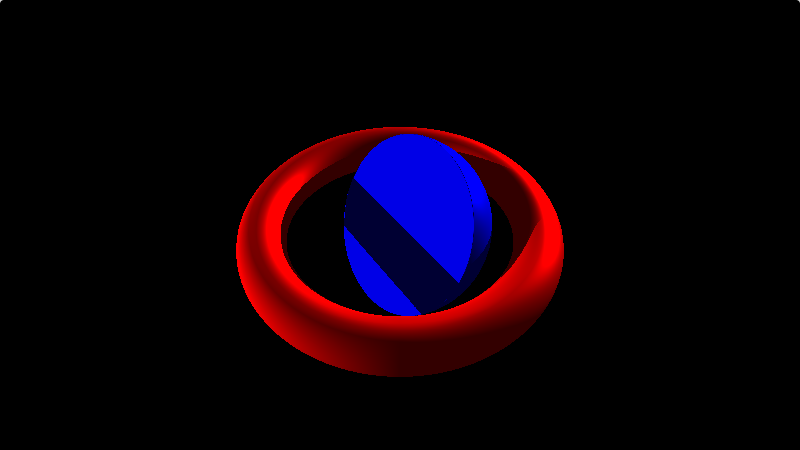
\includegraphics[width=0.8\textwidth]{secciones/imagenes/material/materiales.png}\label{fig:material}
  \caption{Materiales asignados a las distintas figuras.}
\end{figure}